\section{Security of the pipeline}
\label{Security of the pipeline}
Security of the \gls{pipeline} refers to the measures taken to protect the \gls{pipeline} and the underlying infrastructure and network involved in processing the code that passes through it. To ensure the \gls{pipeline} 's security, it is limited to performing its intended functions and stops unauthorized access to restricted resources.

\subsection{Branch Protection}
Branch protection ensures that specific criteria are met before code can be merged \cite{branch}. This feature allows users to create branch protection rules that enforce specific workflows for one or multiple branches, such as mandating an approving review or passing status checks for all pull requests merged into the protected branch. Access to this feature of GitHub is available for all users.
\\~\\
Enforcing branch protection makes introducing errors and vulnerabilities into the secured branch less likely. In addition, branch protection creates a more precise development process by providing guidelines and requirements for making changes in the code. This helps ensure that all team members are aligned towards the same goal and working together effectively.  


\vspace{2mm}
\begin{figure}[H]
    \centering
    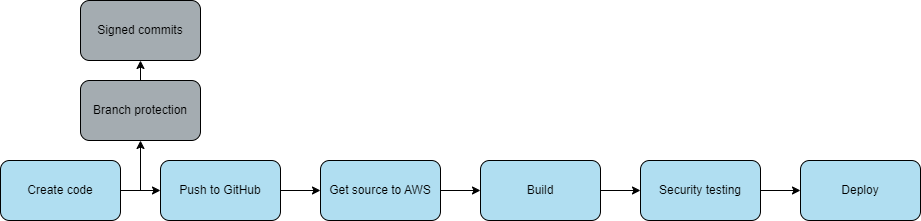
\includegraphics[width=0.8\columnwidth]{Images/pipeline6.png}
    \caption{Pipeline with implemented branch protection rules}
    \label{fig: Pipeline with implemented branch protection rules}
\end{figure}

\subsection{Access Control}
Access control is crucial to regulating individuals' access to specific resources such as GitHub \cite{accesscontroll}. It involves implementing measures to determine the appropriate level of access for each individual while following the \say{least privilege} principle. As specified by \acrshort{nist} \cite{leastprivilege}, this principle entails designing a security architecture, granting each entity only the minimum system resources and authorizations needed to perform its function. 
\\~\\
In GitHub, permissions control access, which refers to the capability to execute specific tasks. In addition, team members can have specific roles assigned to them and specific permissions can be granted to individuals and groups. By following these measures, organizations can effectively manage access control and reduce risks associated with unauthorized access to critical resources. 
\\~\\
Secure authentication is a crucial aspect of maintaining system security \cite{iso27002}. It involves implementing measures to ensure that only authorized users can access a system and that their access is limited to the specific resources needed to perform their duties. Conditional access policies can help organizations improve their authentication process \cite{conditionalaccess}. By specifying specific rules and conditions, the system can determine the appropriate times, locations, and methods for users to gain access. For example, an organization might require multi-factor authentication for all users accessing the system outside the corporate network. In addition, they might limit access to specific applications or data based on the user's role or location.
\newpage
Conditional access is an essential part of an organization's overall security plan. It provides effective system access management, lowering the risk of unwanted access or data breaches and ensuring regulatory compliance. Furthermore, applying this access control to all system components at every pipeline stage is advisable for optimal security, as shown in Figure \ref{fig: Pipeline with implemented access control}. As a result, necessary and consistent access control implementation is crucial.

\vspace{2mm}
\begin{figure}[H]
    \centering
    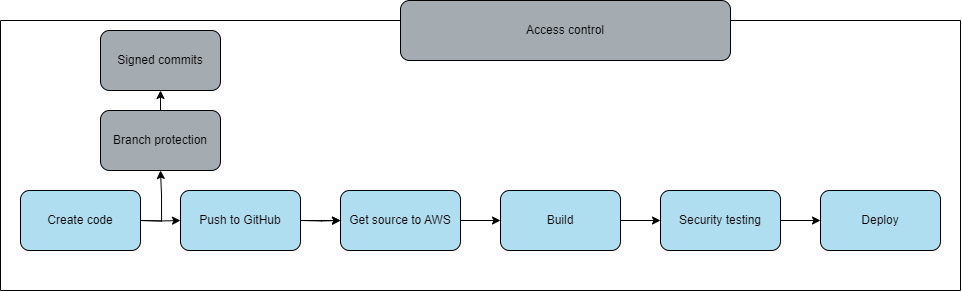
\includegraphics[width=0.8\columnwidth]{Images/accesscontrol.png}
    \caption{Pipeline with implemented access control}
    \label{fig: Pipeline with implemented access control}
\end{figure}

 
\section{Security in maintenance}
Once the deployment process is complete, the application is transferred to the cloud environment in \acrlong{aws} \cite{awsafterdep}. It is essential at this stage to keep the security up to date to ensure that the application and data are protected. \acrshort{aws} offers a range of best practices organizations can follow to decrease risks associated with cloud computing and ensure that the  \acrshort{aws} environment is secure.
\\~\\
After successfully completing the deployment process, it is important to ensure infrastructure security and performance. To solve security problems and offer new features to the system, regular maintenance and upgrades are required. Furthermore, frequent backups and disaster recovery testing are required to protect data and applications. Maintaining and testing the system on a regular basis helps prevent downtime and improve system dependability.
\newpage
It is critical to monitor cloud-based applications continuously in order to discover issues or potential risks  This includes identifying errors, performance problems, safety weaknesses, and other relevant issues. \acrshort{aws} provides specific monitoring tools, such as \acrshort{aws} Cloudtrail\footnote{Available at: \url{https://aws.amazon.com/cloudtrail/}} and \acrshort{aws} X-ray\footnote{Available at: \url{https://aws.amazon.com/xray/}}. 
\\~\\
During the development phases, various security tests, such as security scans and penetration testing, should be done to discover possible vulnerabilities and resolve them before release. However, it is just as critical to do post-deployment testing to ensure that any additional vulnerabilities are found and resolved as soon as possible. Regular security scans and penetration testing can lower the danger of exploitation significantly. By running these tests regularly, a company can keep track of any potential security issues and take preventive measures to mitigate them. 
\\~\\
To ensure that the application is protected, it is recommended that the organization implement a web application firewall like \acrshort{aws} WAF\footnote{Available at: \url{https://aws.amazon.com/waf/}}, to prevent malicious application attacks such as \gls{SQL-injection}, \gls{Cross-site scripting} and other attacks. \acrshort{aws}'s WAF service offers a managed set of protective rules, allowing customized rules and access control lists based on the company's needs and risk models. This makes it possible to provide web application security with more customization and specification. Additionally, it is important to take steps to prevent \gls{ddos} which can be done using \acrshort{aws} Shield\footnote{Available at: \url{https://aws.amazon.com/shield/}}.
\\~\\
Maintaining security is crucial during the maintenance phase of the \acrshort{sdlc}, which starts after the application has been deployed. It is critical to keep up with regular maintenance and testing during this phase and take proactive measures to mitigate any issues that may arise. Organizations can identify and address potential security vulnerabilities beforehand to prevent them from becoming significant issues. This is particularly crucial when deploying applications to the cloud due to the complex and ever-changing security environment. 
\newpage
Best practices such as regular security audits, vulnerability scans, and patches can ensure the application remains secure and protected against potential threats. Monitoring for unusual or suspicious activity can also aid in detecting and preventing security breaches. Organizations can help ensure their \acrshort{aws} applications' continued reliability and security by prioritizing security throughout the maintenance phase.


\section{Finished pipeline}
Figure \ref{fig: Pipeline with all security measures implemented} illustrates a finished pipeline after all security measures are included. This also includes maintenance.  

\vspace{2mm}
\begin{figure}[H]
    \centering
    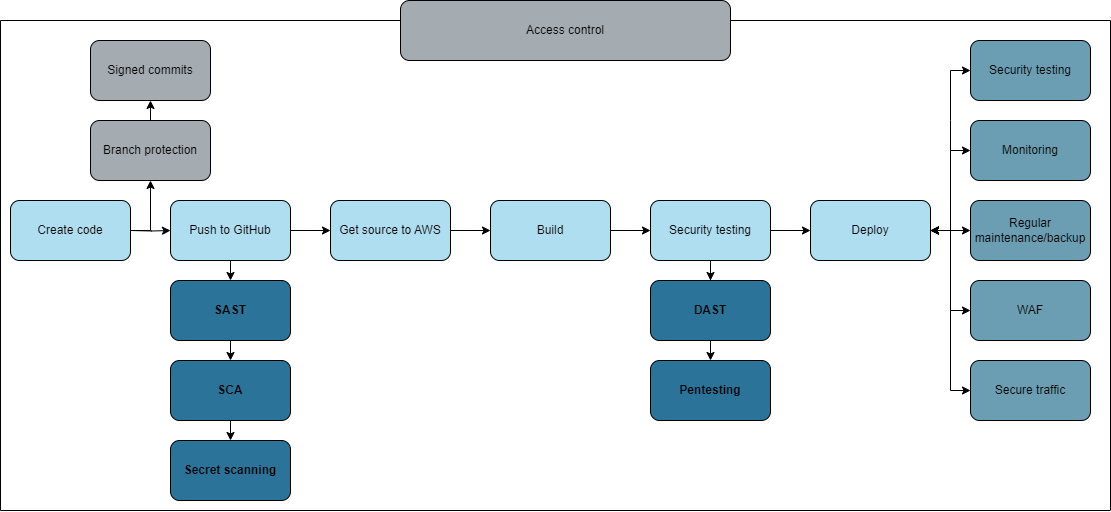
\includegraphics[width=0.8\columnwidth]{Images/FinalPipeline.png}
    \caption{Pipeline with all security measures implemented}
    \label{fig: Pipeline with all security measures implemented}
\end{figure}



